\documentclass{article}

%Aus dem LaTex Template der Universit�t Stuttgart
%------------------------------------------------
\usepackage[utf8]{inputenc}
\usepackage[T1]{fontenc}
\usepackage{cmap}
\usepackage[ngerman]{babel}
\usepackage{graphicx}
\usepackage[pdftex,hyperref,dvipsnames]{xcolor}
\usepackage{listings}
\usepackage[a4paper,lmargin={2cm},rmargin={2cm},tmargin={3.5cm},bmargin = {2.5cm},headheight = {4cm}]{geometry}
\usepackage{amsmath,amssymb,amstext,amsthm}
\usepackage[lined,algonl,boxed]{algorithm2e}
\usepackage{tikz}
\usepackage{hyperref}
\usepackage{url}
\usepackage[inline]{enumitem} % Erm�glicht �ndern der enum Item Zahlen
\usepackage[headsepline]{scrpage2} 
\usepackage{algorithmic} % F�r Pseudocode
\usepackage{ marvosym } % f�r Pfeil(e)
\usepackage{booktabs} % F�r die sch�neren Booktabs-Tabellen
\usepackage{tikz}
\usepackage{pdfpages}
\usepackage{blindtext}
\usepackage{scrextend}
\usepackage{pdfpages}
\usepackage{amsmath}
\usepackage{mathtools}
\pagestyle{scrheadings} 
\usetikzlibrary{automata,positioning,calc,arrows}

\begin{document}
	% Counter für das Blatt und die Aufgabennummer.
% Ersetze die Nummer des Übungsblattes und die Nummer der Aufgabe
% den Anforderungen entsprechend.
% Beachte:
% \setcounter{countername}{number}: Legt den Wert des Counters fest
% \stepcounter{countername}: Erhöht den Wert des Counters um 1.
\newcounter{sheetnr}
\setcounter{sheetnr}{14} % Nummer des Übungsblattes
\newcounter{exnum}
\setcounter{exnum}{1} % Nummer der Aufgabe

% Befehl für die Aufgabentitel
\newcommand{\exercise}[1]{\section*{Aufgabe \theexnum\stepcounter{exnum} #1}} % Befehl für Aufgabentitel

% Formatierung der Kopfzeile
% \ohead: Setzt rechten Teil der Kopfzeile mit
% Namen und Matrikelnummern aller Bearbeiter
\ohead{Lukas Heiland (3269754)\\
	Laura Schuiki (3228407)\\
Barkha Sharma (3290011)}
% \chead{} kann mittleren Kopfzeilen Teil sezten
% \ihead: Setzt linken Teil der Kopfzeile mit
% Modulnamen, Semester und Übungsblattnummer
\ihead{Numerische und stochastische Grundlagen\\
Wintersemester 2017/18\\
Blatt \thesheetnr}
	
	\section*{Aufgabe 2}
		\paragraph*{a)}.
			\begin{figure}[h!]
				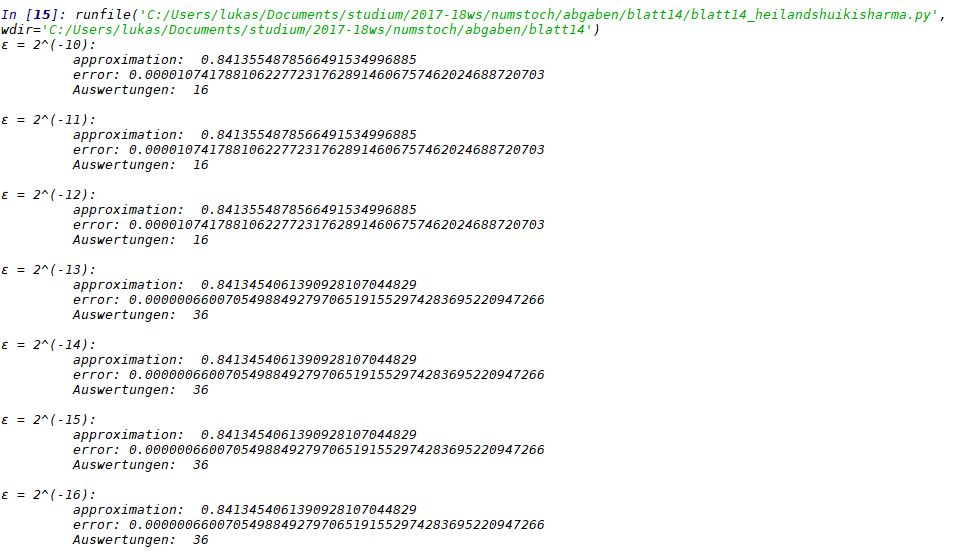
\includegraphics[scale=0.6]{aufgabe2part1.jpg}
				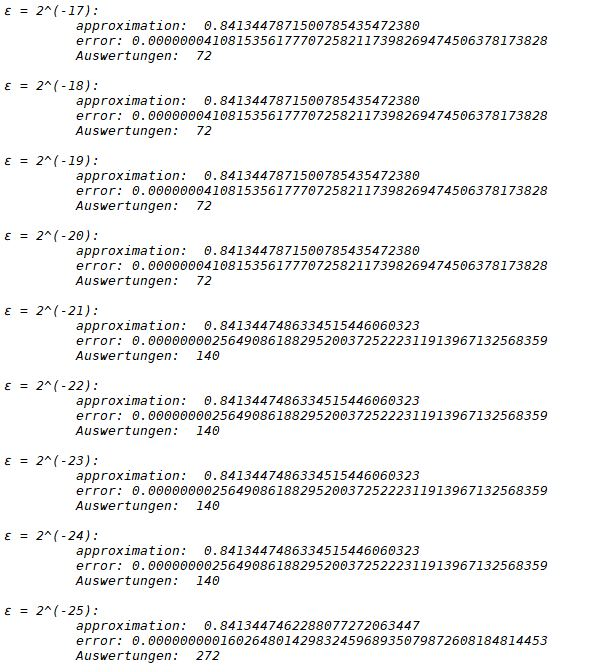
\includegraphics[scale=0.6]{aufgabe2part2.jpg}
				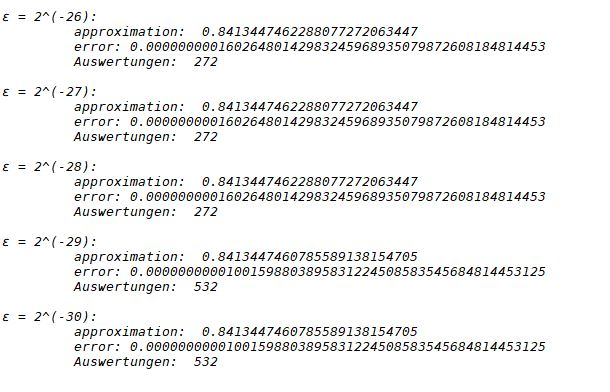
\includegraphics[scale=0.6]{aufgabe2part3.jpg}
			\end{figure}
		\pagebreak
		\paragraph*{b)}.
			\begin{figure}[h!]
				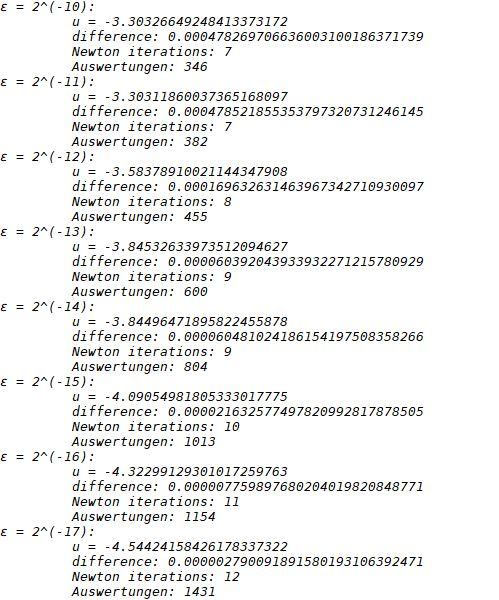
\includegraphics[scale=0.7]{bpart1.jpg}
				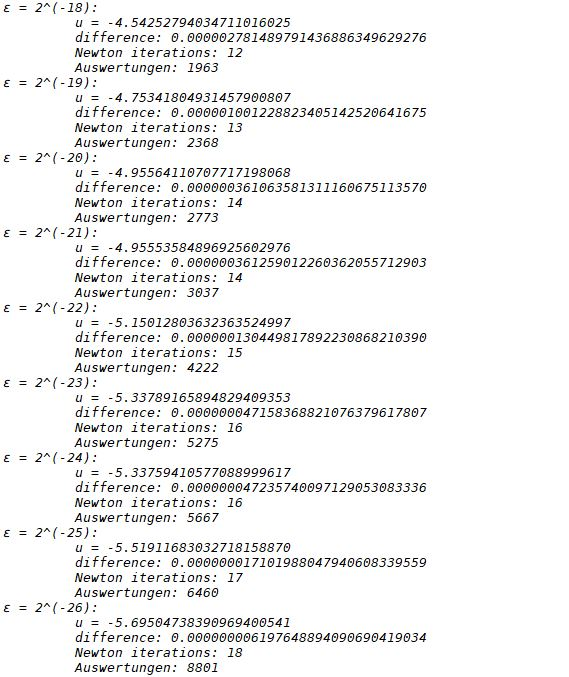
\includegraphics[scale=0.7]{bpart2.jpg}
			\end{figure}
		$2^{-27} \leq \varepsilon \leq 2^{-30}$ auf der nächsten Seite
			\begin{figure}
				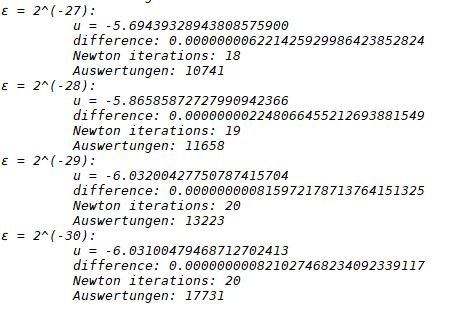
\includegraphics[scale=0.6]{bpart3.jpg}
			\end{figure}
		\pagebreak
		
					%\begin{table}[h]
					%\begin{tabular}{lllr}
					%\textbf{$\varepsilon$} & \textbf{Näherung von $\Phi(1)$} & \textbf{Fehler}   & \multicolumn{1}{l}{\textbf{Auswertungen von $\varphi$}} \\
					%$2^{-10}$            & 0.841872145243                & 0.000527399174928 & 8,193                                                 \\
					%$2^{-11}$            & 0.841608445731                & 0.000263699662581 & 16,385                                                \\
					%$2^{-12}$            & 0.841476595919                & 0.000131849850067 & 32,769                                                \\
					%$2^{-13}$            & 0.841410670998                & 6.59249297345$\cdot 10^{-5}$ & 65,537                                                \\
					%$2^{-14}$            & 0.841377708535                & 3.2962466027$\cdot 10^{-5}$  & 131,073                                               \\
					%$2^{-15}$            & 0.841361227302                & 1.64812333044$\cdot 10^{-5}$ & 262,145                                               \\
					%$2^{-16}$            & 0.841352986685                & 8.24061673221$\cdot 10^{-6}$ & 524,289                                               \\
					%$2^{-17}$            & 0.841348866377                & 4.12030840213$\cdot 10^{-6}$ & 1,048,577                                             \\
					%$2^{-18}$            & 0.841346806223                & 2.06015417292$\cdot 10^{-6}$ & 2,097,153                                             \\
					%$2^{-19}$            & 0.841345776146                & 1.03007711127$\cdot 10^{-6}$ & 4,194,305                                             \\
					%$2^{-20}$            & 0.841345261107                & 5.15038520166$\cdot 10^{-7}$ & 8,388,609                                             \\
					%$2^{-21}$            & 0.841345003588                & 2.57519345293$\cdot 10^{-7}$ & 16,777,217                                            \\
					%$2^{-22}$            & 0.841344874828                & 1.287596193$\cdot 10^{-7}$  & 33,554,433                                            \\
					%$2^{-23}$            & 0.841344810448                & 6.43797478661$\cdot 10^{-8}$ & 67,108,865                                            \\
					%$2^{-24}$            & 0.841344778258                & 3.21899319422$\cdot 10^{-8}$ & 134,217,729                                           \\
					%$2^{-25}$            & 0.841344762163                & 1.60949265027$\cdot 10^{-8}$ & 268,435,457                                           \\
					%$2^{-26}$            & 0.841344738021                & 8.04746325135$\cdot 10^{-9}$  & 536,870,913                                           \\
					%$2^{-27}$            & 0.841344742044                & 4.02373162568$\cdot 10^{-9}$  & 1,073,741,825                                         \\
					%$2^{-28}$            & 0.841344744056                & 2.01186581284$\cdot 10^{-9}$  & 2,147,483,649                                         \\
					%$2^{-29}$            & 0.841344745062                & 1.00593290642$\cdot 10^{-9}$  & 4,294,967,298                                         \\
					%$2^{-30}$            & 0.841344745565                & 5.02966453209$\cdot 10^{-10}$ & 8,589,934,595                                        
					%\end{tabular}
					%\end{table}
		
		
		
		\section*{Aufgabe 4}
			\paragraph*{a)}
				$P_{p_o(0)}(S_2 \leq 0) = P_{p_o(0)}(S_2 = 0) = \beta$............(Kleiner als 0 ist nicht möglich)\\[1.5em]
				
				$\Leftrightarrow \binom{2}{0} \cdot p_o(0)^0 \cdot (1-p_o(0))^2 = \beta$\\[1.1em]
				
				$\Leftrightarrow (1-p_o(0))^2 - \beta = 0$\\[1.1em]
				
				$\Leftrightarrow 1 - 2p_o(0) + p_o(0)^2 - \beta = 0$\\[1.1em]
				
				$\Leftrightarrow p_o(0)^2 - 2p_o(0) + 1 - \beta$\\[1.1em]
				
				das kann man in die Mitternachtsformel einsetzen:\\[1.1em]
				
				$\dfrac{2 \pm \sqrt{4 - 4 \cdot (1 - \beta)}}{2} = \dfrac{2 \pm \sqrt{4\beta}}{2}$\\[1.1em]
				
				$= \dfrac{2 \pm 2\sqrt{\beta}}{2} = 1 \pm \sqrt{\beta}$\\ 
				Da $1 + \sqrt{\beta}$ nicht geht (P wäre dann größer als 1), bleibt nur $1 - \sqrt{\beta}$ übrig.\\[2em]
				
				
				$P_{p_o(1)}(S_2 \leq 1) = \beta$\\[1.1em]
				
				$P_{p_o(1)}(S_2 = 0) + P_{p_o(1)}(S_2 = 1) = \beta$\\[1.1em]
				
				$(1 - p_o(1))^2 + \binom{2}{1} \cdot p_o(1) \cdot (1 - p_o(1)) = \beta$\\[1.1em]
				
				$p_o(1)^2 - 2p_o(1) + 1 + 2\cdot p_o(1) - 2\cdot p_o(1)^2 = \beta$\\[1.1em]
				
				$-p_o(1)^2 + 1 - \beta = 0$\\[1.1em]
				
				Wieder mit der Mitternachtsformel:\\[1.1em]
				
				$\dfrac{0 \pm\sqrt{-4 \cdot (-1) \cdot (1-\beta)}}{-2} =\dfrac{\pm \sqrt{4-4\beta}}{-2}$\\[1.1em]
				
				$= \dfrac{\pm \sqrt{4(1-\beta)}}{-2} = \dfrac{2 \cdot \sqrt{1 - \beta}}{-2} = \pm \sqrt{1-\beta}$\\
				$-\sqrt{1-\beta}$ macht keinen Sinn (P < 0) $\rightarrow \sqrt{1-\beta}$ bleibt übrig.\\[2em]
				
				%%% Laura's Ergänzungen
				$P{p_u(1)}(S_2<1) = 1-\beta\\\\
				P{p_u(1)}(S_2\leq 0) = 1-\beta\\\\
				(1-P{p_u(1)})^2= 1-\beta\\\\
				p_u(1)^2 - 2p_u(1) +\beta= 0\\\\
				Mitternachtsformel\Rightarrow \frac{2\pm\sqrt{(14-4*1*\beta)}}{2}\\\\
				\Rightarrow 1\pm \sqrt{1-\beta}\\\\
				Ergebnis: 1- \sqrt{1-\beta}\\\\
				$
				$P{p_u(2)}(S_2<2) = 1-\beta\\\\
				P{p_u(2)}(S_2\leq 1) = 1-\beta\\\\
				-p_u(2)^2 +\beta= 0\\\\
				Mitternachtsformel \Rightarrow \frac{\pm\sqrt{(-4(-1)+\beta)}}{-2}\\\\
				\Rightarrow \pm \sqrt{\beta}\\\\
				Ergebnis: + \sqrt{\beta}\\$ 
				Nur ein Ergebnis, da das Ergebnis nicht negativ sein darf!
				
				
				  

\end{document}